\documentclass{article}[18pt]
%\ProvidesPackage{format}
%Page setup
\usepackage[utf8]{inputenc}
\usepackage[margin=0.7in]{geometry}
\usepackage{parselines} 
\usepackage[english]{babel}
\usepackage{fancyhdr}
\usepackage{titlesec}
\hyphenpenalty=10000

\pagestyle{fancy}
\fancyhf{}
\rhead{Sam Robbins}
\rfoot{Page \thepage}

%Characters
\usepackage{amsmath}
\usepackage{amssymb}
\usepackage{gensymb}
\newcommand{\R}{\mathbb{R}}

%Diagrams
\usepackage{pgfplots}
\usepackage{graphicx}
\usepackage{tabularx}
\usepackage{relsize}
\pgfplotsset{width=10cm,compat=1.9}
\usepackage{float}

%Length Setting
\titlespacing\section{0pt}{14pt plus 4pt minus 2pt}{0pt plus 2pt minus 2pt}
\newlength\tindent
\setlength{\tindent}{\parindent}
\setlength{\parindent}{0pt}
\renewcommand{\indent}{\hspace*{\tindent}}

%Programming Font
\usepackage{courier}
\usepackage{listings}
\usepackage{pxfonts}

%Lists
\usepackage{enumerate}
\usepackage{enumitem}

% Networks Macro
\usepackage{tikz}


% Commands for files converted using pandoc
\providecommand{\tightlist}{%
	\setlength{\itemsep}{0pt}\setlength{\parskip}{0pt}}
\usepackage{hyperref}

% Get nice commands for floor and ceil
\usepackage{mathtools}
\DeclarePairedDelimiter{\ceil}{\lceil}{\rceil}
\DeclarePairedDelimiter{\floor}{\lfloor}{\rfloor}

% Allow itemize to go up to 20 levels deep (just change the number if you need more you madman)
\usepackage{enumitem}
\setlistdepth{20}
\renewlist{itemize}{itemize}{20}

% initially, use dots for all levels
\setlist[itemize]{label=$\cdot$}

% customize the first 3 levels
\setlist[itemize,1]{label=\textbullet}
\setlist[itemize,2]{label=--}
\setlist[itemize,3]{label=*}

% Definition and Important Stuff
% Important stuff
\usepackage[framemethod=TikZ]{mdframed}

\newcounter{theo}[section]\setcounter{theo}{0}
\renewcommand{\thetheo}{\arabic{section}.\arabic{theo}}
\newenvironment{important}[1][]{%
	\refstepcounter{theo}%
	\ifstrempty{#1}%
	{\mdfsetup{%
			frametitle={%
				\tikz[baseline=(current bounding box.east),outer sep=0pt]
				\node[anchor=east,rectangle,fill=red!50]
				{\strut Important};}}
	}%
	{\mdfsetup{%
			frametitle={%
				\tikz[baseline=(current bounding box.east),outer sep=0pt]
				\node[anchor=east,rectangle,fill=red!50]
				{\strut Important:~#1};}}%
	}%
	\mdfsetup{innertopmargin=10pt,linecolor=red!50,%
		linewidth=2pt,topline=true,%
		frametitleaboveskip=\dimexpr-\ht\strutbox\relax
	}
	\begin{mdframed}[]\relax%
		\centering
		}{\end{mdframed}}



\newcounter{lem}[section]\setcounter{lem}{0}
\renewcommand{\thelem}{\arabic{section}.\arabic{lem}}
\newenvironment{definition}[1][]{%
	\refstepcounter{lem}%
	\ifstrempty{#1}%
	{\mdfsetup{%
			frametitle={%
				\tikz[baseline=(current bounding box.east),outer sep=0pt]
				\node[anchor=east,rectangle,fill=blue!20]
				{\strut Definition};}}
	}%
	{\mdfsetup{%
			frametitle={%
				\tikz[baseline=(current bounding box.east),outer sep=0pt]
				\node[anchor=east,rectangle,fill=blue!20]
				{\strut Definition:~#1};}}%
	}%
	\mdfsetup{innertopmargin=10pt,linecolor=blue!20,%
		linewidth=2pt,topline=true,%
		frametitleaboveskip=\dimexpr-\ht\strutbox\relax
	}
	\begin{mdframed}[]\relax%
		\centering
		}{\end{mdframed}}
	
\newcounter{prob}[section]\setcounter{prob}{0}
\renewcommand{\theprob}{\arabic{section}.\arabic{lem}}
\newenvironment{problem}[1][]{%
	\refstepcounter{prob}%
	\ifstrempty{#1}%
	{\mdfsetup{%
			frametitle={%
				\tikz[baseline=(current bounding box.east),outer sep=0pt]
				\node[anchor=east,rectangle,fill=orange!20]
				{\strut Problem};}}
	}%
	{\mdfsetup{%
			frametitle={%
				\tikz[baseline=(current bounding box.east),outer sep=0pt]
				\node[anchor=east,rectangle,fill=orange!20]
				{\strut Problem:~#1};}}%
	}%
	\mdfsetup{innertopmargin=10pt,linecolor=orange!20,%
		linewidth=2pt,topline=true,%
		frametitleaboveskip=\dimexpr-\ht\strutbox\relax
	}
	\begin{mdframed}[]\relax%
	}{\end{mdframed}}
	
% Styling Pseudocode
\lstset{language=C,
	basicstyle=\ttfamily,
	keywordstyle=\bfseries,
	showstringspaces=false,
	morekeywords={if, else, then, print, end, for, do, while, Let},
	tabsize=4,
	mathescape=true,
	escapechar=£,
	numbers=left,
	stepnumber=1,
	frame=top,
	frame=bottom
}

\usepackage{caption}
\DeclareCaptionFormat{listing}{\rule{\dimexpr\textwidth+17pt\relax}{0.4pt}\par\vskip1pt#1#2#3}
\captionsetup[lstlisting]{format=listing,singlelinecheck=false, margin=0pt, font={sf},labelsep=space,labelfont=bf}


% Mathscr font
\usepackage{mathrsfs}

% Ensures there's a bit of the section before a new page
\preto{\subsection}{\Needspace{5\baselineskip}}
\preto{\section}{\Needspace{5\baselineskip}}
\lhead{AZ900}


\begin{document}
\begin{center}
\underline{\huge Security, responsibility and trust in Azure}
\end{center}
\section{Shared responsibility of cloud security}
\begin{center}
	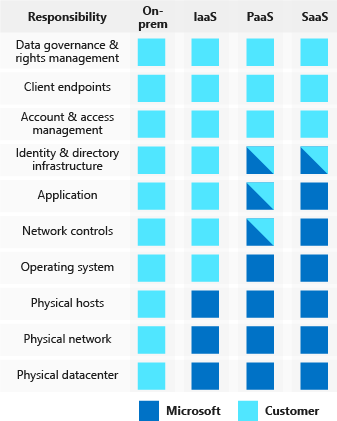
\includegraphics[width=7cm]{2-shared_responsibilities}
\end{center}
Regardless of the deployment type, you always retain responsibility for:
\begin{itemize}
	\item Data
	\item Endpoints
	\item Accounts
	\item Access Management
\end{itemize}
\subsection{Layered approach to security}
\subsubsection{Data}
It is the responsibility of those storing and controlling access to the data to ensure that it's properly secured. There are often regulatory requirements for the CIA of this data
\subsubsection{Application}
\begin{itemize}
	\item Ensure applications are secure and free of vulnerabilities
	\item Store sensitive application secrets in a secure storage medium
	\item Make security a design requirement for all application development
\end{itemize}
\subsubsection{Compute}
\begin{itemize}
	\item Secure access to virtual machines
	\item Implement endpoint protection and keep systems patched and current
\end{itemize}
\subsubsection{Networking}
\begin{itemize}
	\item Limit communication between resources
	\item Deny by default
	\item Restrict inbound internet access and limit outbound, where appropriate
	\item Implement secure connectivity to on-premises networks
\end{itemize}
\subsection{Perimeter}
\begin{itemize}
	\item Use DDoS protection
	\item Use perimeter firewalls to identify and alert on malicious attacks against your network
\end{itemize}
\subsection{Identity and access}
\begin{itemize}
	\item Control access to infrastructure and change control
	\item Use single sign on and multi factor authentication
	\item Audit events and changes
\end{itemize}
\subsection{Physical security}
\begin{itemize}
	\item Physical building security and controlling access to computing hardware within the data center is the first line of defence
\end{itemize}
\section{Azure Security Center}
Security Center can:
\begin{itemize}
	\item Provide security recommendations based on your configurations, resources and networks
	\item Monitor security settings and automatically apply required security to new services
	\item Continuously monitor services to provide automatic security assessments
	\item Use machine learning to detect and block malware being installed
	\item Analyse and identify inbound attacks
	\item Provide just in time access control for ports
\end{itemize}
\subsection{Pricing Tiers}
\begin{itemize}
	\item Free - Just assessments and recommendations of resources
	\item Standard - Including continuous monitoring, threat detection etc.
\end{itemize}
\subsection{Usage scenarios}
You can use security centre to:
\begin{itemize}
	\item Detect - Review the first indication of an event investigation
	\item Assess - Perform the initial assessment to obtain more information about the suspicious activity
	\item Implement a recommended security policy
\end{itemize}

\section{Identity and access}
\begin{definition}[Authentication]
	Establish the identity of a person or service looking to access a resource
\end{definition}
\begin{definition}[Authorization]
	Establish what level of access an authenticated person or service has
\end{definition}
\subsection{Azure Active Directory}
Azure AD provides services such as:
\begin{itemize}
	\item Authentication
	\item Single Sign On - One ID and password for multiple services
	\item Application management
	\item Business to Business identity services
	\item Business to Customer identity services
	\item Device management
\end{itemize}
\subsection{Providing identities to services}
\subsubsection{Service Principals}
\begin{definition}[Identity]
	A thing that can be authenticated
\end{definition}
\begin{definition}[Principal]
	An identity acting with certain roles or claims
\end{definition}
\begin{definition}[Service Principal]
	An identity that is used by a service or application
\end{definition}
\subsubsection{Managed identities for Azure services}
This makes creating service principles easier. A managed identity can be instantly created for any azure service that supports it. 
\subsection{Role based access control}
Roles are sets of permissions that users can be granted to access an Azure service instance.\\
\\
Identities are mapped to roles directly or through group membership.\\
\\
Roles can be granted at the individual service instance level, but they also flow down the Azure resource manager hierarchy.
\subsubsection{Privileged Identity Management}
This is an additional offering that provides oversight of role assignments to ensure people don't hav excess privileges. 
\section{Encryption}
\begin{definition}[Symmetric encryption]
	Uses the same key to encrypt and decrypt the data
\end{definition}
\begin{definition}[Asymmetric encryption]
	Uses a public and private key pair
\end{definition}
\begin{definition}[Encryption at rest]
	Encrypting data that has been stored on a physical medium
\end{definition}
\begin{definition}[Encryption in transit]
	Encrypting data that is actively moving from one location to another
\end{definition}
\subsection{Encryption on Azure}
\begin{itemize}
	\item Azure Storage Service Encryption - For data at rest
	\item Azure Disk Encryption - Encrypt virtual machine disks
	\item Transparent data encryption - Protect Azure SQL database and Azure data warehouse
	\item Azure key vault - encrypt secrets
\end{itemize}
Benefits of using key vault:
\begin{itemize}
	\item Centralized application secrets
	\item Securely stored secrets and keys
	\item Monitor access and use
	\item Simplified administration of application secrets
	\item Integrate with other Azure services
\end{itemize}
\section{Azure Certificates}
Certificates in Azure are \textbf{x.509 v3} and can be signed by a CA or self signed
\subsection{Service Certificates}
These are attached to cloud services and enable secure communication to and from this service.\\
\\
These are managed separately from the services.
\subsection{Management certificates}
These allow you to authenticate with the classic deployment model 
\section{Protect your network}
\begin{definition}[Firewall]
	A service that grants server access based on the originating IP address of each request
\end{definition}
To provide inbound protection at the perimeter, you have several choices:
\begin{itemize}
	\item Azure firewall - Managed cloud based network security service
	\item Azure application gateway - Load balancer that includes a web application firewall
	\item Network virtual appliances (NVAs) - Ideal for non HTTP services or advanced configs
\end{itemize}
\subsection{DDoS Protection}
Basic:
\begin{itemize}
	\item Automatically enabled
	\item Always on traffic monitoring and real time mitigation of common network level attcks
\end{itemize}
Standard:
\begin{itemize}
	\item Can mitigate:
	\begin{itemize}
		\item Volumetric attacks - Flooding network layer with traffic
		\item Protocol attacks - Exploit weakness in layer 3 and layer 4 protocol stack
		\item Resource layer attacks - Target web application packets to disrupt the transmission of data between hosts
	\end{itemize}
\end{itemize}
\subsection{Virtual network security}
For communication between virtual machines, Network Security Groups are a critical piece to restrict unnecessary communication.\\
\\
This allows you to filter network traffic to and from Azure resources in an Azure virtual network
\subsection{Network Integration}
To provide a dedicated private network between your network and Azure, you can use Azure ExpressRoute.
\section{Protecting shared documents}
Azure information protection - A cloud based solution to help organizations classify and optionally protect documents by applying labels
\section{Azure Advanced Threat Protection}
This is a cloud based solution to identify, detect and help to investigate threats.\\
\\
It has the following components:
\begin{itemize}
	\item ATP portal - Allows you to monitor and respond to suspicious activity
	\item ATP sensor - Installed directly on domain controllers to monitor traffic
	\item ATP cloud service - Runs on Azure infrastructure and is connected to Microsoft's intelligent security graph
\end{itemize}
\section{Security considerations for Application Lifecycle Management Solutions}
\begin{itemize}
	\item Provide training to ensure everyone knows the threats
	\item Define security requirements - Update continuously to address change in threat landscape. 
	\item Define metrics and compliance reporting - Have minimum levels of security quality
	\item Perform threat modelling - Allows development teams to consider the security implications of designs
	\item Establish design requirements - Specific security features must be implemented
	\item Define and use cryptography standards
	\item Manage security risks from using third-party components - Keep an accurate inventory and plan to respond when new vulnerabilities are discovered
	\item Use approved tools - Define and publish a list of approved tools
	\item Perform Static Analysis Security Testing - Analyse source code prior to compilation
	\item Perform Dynamic Analysis Security Testing - Analyse fully compiled code
	\item Perform penetration testing
	\item Establish a standard incident response process
\end{itemize}
\end{document}
